\documentclass{article}[twocolumn]
\usepackage[pdftex]{graphicx}
\usepackage[utf8]{inputenc}
\usepackage[brazil]{babel}
\usepackage{subfigure}
\usepackage{mathtools}
\usepackage{amsmath}
\usepackage{amssymb}
\usepackage{float}
\usepackage{tikz}
\usepackage[a4paper,top=2.5cm,bottom=2.5cm,left=2cm,right=2cm,marginparwidth=1.5cm]{geometry}

\title{Relat\'orio da pr\'atica 2}
\author{Kenji Yamane}

\begin{document}
	\maketitle
	\section{Quest\~ao 1}
	Query:
	\begin{verbatim}
		SELECT last_name, salary FROM employees WHERE salary > 12000;
	\end{verbatim}
	Print:
	\begin{figure}[H]
		\centering
		\includegraphics[width=\textwidth]{images/questao1.png}
	\end{figure}
	\newpage
	\section{Quest\~ao 2}
	Query:
	\begin{verbatim}
		SELECT last_name, department_id
		FROM employees WHERE employee_id = '176';
	\end{verbatim}
	Print:
	\begin{figure}[H]
		\centering
		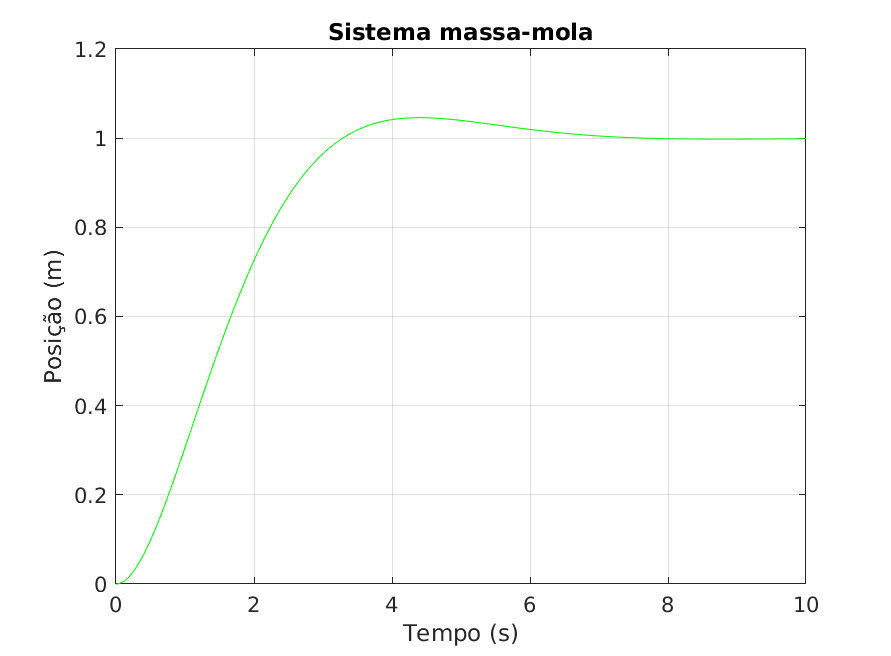
\includegraphics[width=\textwidth]{images/questao2.png}
	\end{figure}
	\newpage
	\section{Quest\~ao 3}
	Query:
	\begin{verbatim}
		SELECT last_name, salary
		FROM employees WHERE salary BETWEEN 5000 AND 12000;
	\end{verbatim}
	Print:
	\begin{figure}[H]
		\centering
		\includegraphics[width=\textwidth]{images/questao3.png}
	\end{figure}
	\newpage
	\section{Quest\~ao 4}
	Query:
	\begin{verbatim}
		SELECT last_name, job_id, hire_date
		FROM employees WHERE last_name IN ('Matos', 'Taylor')
		ORDER BY hire_date;
	\end{verbatim}
	Print:
	\begin{figure}[H]
		\centering
		\includegraphics[width=\textwidth]{images/questao4.png}
	\end{figure}
	\newpage
	\section{Quest\~ao 5}
	Query:
	\begin{verbatim}
		SELECT last_name, department_id
		FROM employees WHERE department_id IN (20, 50)
		ORDER BY CONCAT(first_name, last_name);
	\end{verbatim}
	Print:
	\begin{figure}[H]
		\centering
		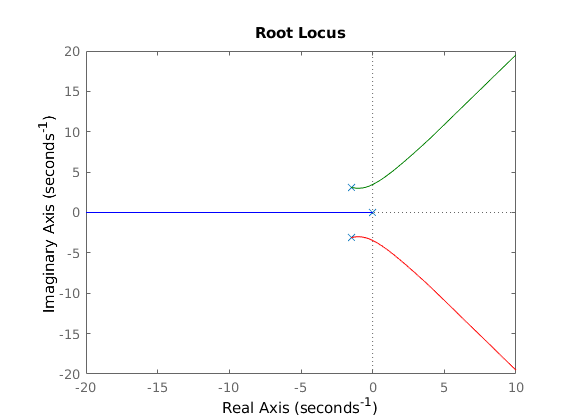
\includegraphics[width=\textwidth]{images/questao5.png}
	\end{figure}
	\newpage
	\section{Quest\~ao 6}
	Query:
	\begin{verbatim}
		SELECT last_name "Empregado", salary "Salário Mensal"
		FROM employees
		WHERE salary BETWEEN 5000 AND 12000
		AND department_id IN (20, 50);
	\end{verbatim}
	Print:
	\begin{figure}[H]
		\centering
		\includegraphics[width=\textwidth]{images/questao6.png}
	\end{figure}
	\newpage
	\section{Quest\~ao 7}
	Query:
	\begin{verbatim}
		SELECT last_name, hire_date FROM employees
		WHERE DATEPART(yyyy, hire_date) = 2002;
	\end{verbatim}
	Print:
	\begin{figure}[H]
		\centering
		\includegraphics[width=\textwidth]{images/questao7.png}
	\end{figure}
	\newpage
	\section{Quest\~ao 8}
	Query:
	\begin{verbatim}
		SELECT employees.last_name, jobs.job_title
		FROM employees
		LEFT JOIN jobs ON employees.job_id = jobs.job_id
		WHERE employees.manager_id IS NULL;
	\end{verbatim}
	Print:
	\begin{figure}[H]
		\centering
		\includegraphics[width=\textwidth]{images/questao8.png}
	\end{figure}
	\newpage
	\section{Quest\~ao 9}
	Query:
	\begin{verbatim}
		SELECT last_name, salary, commission_pct
		FROM employees
		WHERE commission_pct IS NOT NULL
		ORDER BY salary DESC, commission_pct DESC;
	\end{verbatim}
	Print:
	\begin{figure}[H]
		\centering
		\includegraphics[width=\textwidth]{images/questao9.png}
	\end{figure}
	\newpage
	\section{Quest\~ao 10}
	Query:
	\begin{verbatim}
		SELECT last_name, salary FROM employees
		WHERE salary > $(salary_lower_threshold);
	\end{verbatim}
	Print:
	\begin{figure}[H]
		\centering
		\includegraphics[width=\textwidth]{images/questao10.png}
	\end{figure}
	\newpage
	\section{Quest\~ao 11}
	Query:
	\begin{verbatim}
		SELECT last_name FROM employees
		WHERE last_name LIKE '__a%';
	\end{verbatim}
	Print:
	\begin{figure}[H]
		\centering
		\includegraphics[width=\textwidth]{images/questao11.png}
	\end{figure}
	\newpage
	\section{Quest\~ao 12}
	Query:
	\begin{verbatim}
		SELECT last_name FROM employees
		WHERE last_name LIKE '%a%e%'
		OR last_name LIKE '%e%a%';
	\end{verbatim}
	Print:
	\begin{figure}[H]
		\centering
		\includegraphics[width=\textwidth]{images/questao12.png}
	\end{figure}
	\newpage
	\section{Quest\~ao 13}
	Query:
	\begin{verbatim}
		SELECT last_name, job_id, salary FROM employees
		WHERE job_id IN ('SA_REP', 'ST_MAN')
		AND salary NOT IN (2500, 3500, 7000);
	\end{verbatim}
	Print:
	\begin{figure}[H]
		\centering
		\includegraphics[width=\textwidth]{images/questao13.png}
	\end{figure}
	\newpage
	\section{Quest\~ao 14}
	Query:
	\begin{verbatim}
		SELECT last_name,
		COALESCE(CONVERT(VARCHAR(10), commission_pct), 'Sem Comissão') "COMISSAO"
		FROM employees;
	\end{verbatim}
	Print:
	\begin{figure}[H]
		\centering
		\includegraphics[width=\textwidth]{images/questao14.png}
	\end{figure}
	\newpage
	\section{Quest\~ao 15}
	Query:
	\begin{verbatim}
		SELECT last_name, salary, commission_pct
		FROM employees WHERE commission_pct = 0.2;
	\end{verbatim}
	Print:
	\begin{figure}[H]
		\centering
		\includegraphics[width=\textwidth]{images/questao15.png}
	\end{figure}
	\newpage
	\section{Quest\~ao 16}
	Query:
	\begin{verbatim}
		SELECT CURRENT_TIMESTAMP "Data de Hoje";
	\end{verbatim}
	Print:
	\begin{figure}[H]
		\centering
		\includegraphics[width=\textwidth]{images/questao16.png}
	\end{figure}
	\newpage
	\section{Quest\~ao 17}
	Query:
	\begin{verbatim}
		SELECT employee_id, last_name, salary, FLOOR(salary*1.155) FROM employees;
	\end{verbatim}
	Print:
	\begin{figure}[H]
		\centering
		\includegraphics[width=\textwidth]{images/questao17.png}
	\end{figure}
	\newpage
	\section{Quest\~ao 18}
	Query:
	\begin{verbatim}
		SELECT last_name, hire_date, DATEPART(dw, hire_date) "DIA DA SEMANA ADMISSÃO"
		FROM employees ORDER BY "DIA DA SEMANA ADMISSÃO";
	\end{verbatim}
	Print:
	\begin{figure}[H]
		\centering
		\includegraphics[width=\textwidth]{images/questao18.png}
	\end{figure}
	\newpage
	\section{Quest\~ao 19}
	Query:
	\begin{verbatim}
		SELECT last_name,
		ROUND(DATEDIFF(month, hire_date, CURRENT_TIMESTAMP), 0) "MESES_TRABALHADOS"
		FROM employees ORDER BY "MESES_TRABALHADOS";
	\end{verbatim}
	Print:
	\begin{figure}[H]
		\centering
		\includegraphics[width=\textwidth]{images/questao19.png}
	\end{figure}
	\newpage
	\section{Quest\~ao 20}
	Query:
	\begin{verbatim}
		SELECT LEFT(last_name, 8) + ' '
		+ CONVERT(VARCHAR(10), CEILING(salary)) "EMPLOYEES_AND_SALARIES"
		FROM employees ORDER BY salary DESC;
	\end{verbatim}
	Print:
	\begin{figure}[H]
		\centering
		\includegraphics[width=\textwidth]{images/questao20.png}
	\end{figure}
\end{document}
